%\documentclass[12pt]{article}%

%%%%%%%%%%%######################################### MASTER FILE ###############################################


%\documentclass[12pt]{article}%
\usepackage{amssymb, amsfonts, amsmath}
\usepackage{mathrsfs}
\usepackage{graphicx}
\usepackage[usenames,dvipsnames]{xcolor}
\usepackage{tikz}
\usepackage{float}
\usepackage{enumitem}
\usepackage{comment}
\usepackage{setspace}
\usepackage{caption}
\usepackage{subcaption}
\usepackage[hidelinks]{hyperref}
\usepackage{array}%
%\usepackage{eufrak}
\usepackage{multicol}

\setcounter{MaxMatrixCols}{30}%

\newcolumntype{C}[1]{>{\centering\let\newline\\\arraybackslash\hspace{0pt}}m{#1}}
\providecommand{\U}[1]{\protect\rule{.1in}{.1in}}
\providecommand{\boksie}{\ensuremath{\mathbin{\raisebox{0.3mm}{$\scriptstyle\square$}}}}

% -- DIMENSIONS --
\textwidth=6.4in
\textheight=9in
\evensidemargin=0in
\oddsidemargin=0in
\topmargin=-0.6in
\topskip=0pt
\baselineskip=12pt
\parskip=2mm

\begin{comment}
\newtheorem{theorem}{Theorem}
\newtheorem{acknowledgment}[theorem]{Acknowledgment}  
\newtheorem{algo}{Algorithm}
\newtheorem{axiom}[theorem]{Axiom}
\newtheorem{case}[theorem]{Case}
\newtheorem{claim}[theorem]{Claim}
\newtheorem{conclusion}[theorem]{Conclusion}
\newtheorem{condition}[theorem]{Condition}
\newtheorem{conj}{Conjecture}
\newtheorem{cons}[theorem]{Construction}
\newtheorem{coro}[theorem]{Corollary}
\newtheorem{criterion}[theorem]{Criterion}
\newtheorem{defn}[theorem]{Definition}
\newtheorem{exercise}[theorem]{Exercise}
\newtheorem{lemma}[theorem]{Lemma}
\newtheorem{notation}[theorem]{Notation}
\newtheorem{obs}[theorem]{Observation}
\newtheorem{problem}{Problem}
\newtheorem{prop}[theorem]{Proposition}
\newtheorem{remark}[theorem]{Remark}
\newtheorem{solution}[theorem]{Solution}
\newtheorem{summary}[theorem]{Summary}
\end{comment}

%\newenvironment{proof}[1][Proof]{\noindent\textbf{#1.} }{\ \hfill \rule{0.5em}{0.5em}}
%\renewenvironment{proof}[1][Proof]{\noindent\textbf{#1.} }{\ \hfill \rule{0.5em}{0.5em}}

%--------------------------COMMANDS -------------------------------------------------


%%% Notes to self: %%%
%\newcommand{\nts}[1]{{ \noindent \color{blue} \vspace{5mm} {\bf **NOTE** }  #1}}
\newcommand{\nts}[1]{{ \noindent \color{blue} {\bf **NOTE** }  #1}}
\newcommand{\pr}[1]{{ \color{ForestGreen} [{\bf PR: }  #1]}}
\newcommand{\cmty}[1]{{\color{Fuchsia}(#1)}}
\newcommand{\ft}[1]{{\color{red}#1}}

%%% Math Shortcuts  %%%
\newcommand{\Mod}[1]{\ (\text{mod}\ #1)}
%\newcommand{\ig}[1]{#1(i)}
%\newcommand{\ig}[1]{\mathswab{I}(#1)}
\newcommand{\ig}[1]{\mathscr{I}(#1)}
\newcommand{\agraph}{\alpha}
\newcommand{\ag}[1]{\mathscr{A}(#1)}
\newcommand{\cp}[1]{\overline{#1}}
\newcommand{\thet}[1]{\Theta\left\langle #1\right\rangle }


\providecommand{\diam}{\operatorname{diam}}
\providecommand{\rad}{\operatorname{rad}}
\providecommand{\dist}{\operatorname{dist}}
\providecommand{\bm}{\boldsymbol}
%\renewcommand{\mod}{\operatorname{mod}\ }
%\renewcommand{\vec}[1]{\mathbf{#1}}
\providecommand{\pn}{\operatorname{pn}}
\providecommand{\gid}{\gamma^{ID}}
\providecommand{\ggid}{G(\gamma^{ID})}
\providecommand{\leqn}{1 \leq i \leq n}
\providecommand{\gpr}{\gamma_{pr}}
\providecommand{\gt}{\gamma_{t}}
\providecommand{\ir}{\operatorname{ir}}

%--- manual proof slug
\providecommand{\slug}{\rule{0.5em}{0.5em}}

%--- special graphs
\providecommand{\bull}{\mathcal{B}}
\newcommand{\Dia}{\mathfrak{D}}
\newcommand{\house}{\mathcal{H}}
\newcommand{\wlat}{\mathfrak{L}}
\newcommand{\bcl}{\mathfrak{B}}
\newcommand{\ntni}{\mathfrak{T}}

%--- Notation for cycle i-graphs
\newcommand{\cid}[1]{\left\langle #1 \right\rangle }
\newcommand{\bk}[1]{\left\lbrace  #1 \right\rbrace  }


%%% Common Graph Things  
\newcommand{\dual}[1]{\widetilde{#1}}


%%% 2-part work around for \edge definition.  No idea how it works.  Why do you do this to yourself?
%- 4 parameter - X,x,y,Y - version
\def\ieInner(#1,#2,#3,#4){#1 \overset{#2 #3}{\sim} #4}
\def\edge#1{\ieInner(#1)}
%
%- 3 parameter - X,x,y - mid list - version
\def\ieInnerA(#1,#2,#3){\overset{#1 #2}{\sim} #3}
\def\adedge#1{\ieInnerA(#1)}
\def\sedge(#1,#2){#1\sim #2}
%
%- 5 parameter - X,x,y,Y,G - version
%\def\ieInnerB(#1,#2,#3,#4,#5){#1 \underset{#5}{\overset{#2 #3}{\sim}} #4} %True Under Version
\def\ieInnerB(#1,#2,#3,#4,#5){#1 \overset{#2 #3}{\sim_{#5}} #4} %Under to side version
\def\edgeG#1{\ieInnerB(#1)}
%
%- 3 parameter - X,Y,G - version
\def\ieInnerC(#1,#2,#3){#1 {\sim_{#3}} #2 }
\def\adjG#1{\ieInnerC(#1)}
%
%-  parameter - X1,X2,...Xk - version
\def\ieInnerD(#1,#2,#3,#4){#1 \sim #2 \sim \dots \sim #3 \sim #4}
\def\adjL#1{\ieInnerD(#1)}
%
%- no inner parameter X~Y version
\def\ieInnerE(#1,#2){#1 \sim #2}
\def\onlyedge#1{\ieInnerE(#1)}

%- tilde only version
\def\ieInnerF(#1,#2){\overset{#1 #2}{\sim}}
\def\onlyTilde#1{\ieInnerF(#1)}


%%% HELP %%% \providecommand defines a new command if it isn't already defined.
%%% HELP %%% \newcommand defines a new command, and makes an error if it is already defined.
%%% HELP %%% \renewcommand redefines a predefined command, and makes an error if it is not yet defined.

%+++++ Custom Colours ++++
\definecolor{ltsky}{RGB}{0,191,255}
\definecolor{ltteal}{RGB}{0, 128, 128 }
\definecolor{medOrch}{RGB}{122,55,139}
\definecolor{royalBlue}{RGB}{65,105,225}
\definecolor{forGreen}{RGB}{34,139,34}
\definecolor{dand}{RGB}{255,193,37}
\definecolor{lightBlue}{RGB}{176,226,255}
\definecolor{lgrey}{RGB}{209,209,209}
\definecolor{lgray}{gray}{0.95}
\definecolor{mgray}{gray}{0.40}
\definecolor{mmgray}{gray}{0.60}
\definecolor{zelim}{RGB}{7,163,82}
\definecolor{zelim2}{RGB}{5,114,57}


%++++ TIKZ  GARBAGE ++++
\usetikzlibrary{fit,positioning,calc, arrows, shapes}
\usetikzlibrary{decorations.pathreplacing}
\usetikzlibrary{backgrounds}
%\usetikzlibrary{patterns}
%\usetikzlibrary{intersections}
%\usepackage{pgfplots}
\tikzstyle{std}=[ circle, draw=black,fill=black,thick, inner sep=2pt, minimum size=2.5mm]
\tikzstyle{wstd}=[ circle, draw=black,fill=white,thick, inner sep=2pt, minimum size=2.5mm]
\tikzstyle{ir}=[ circle, draw=black,fill=green,thick,  inner sep=2pt, minimum size=2mm]
\tikzstyle{mp}=[circle, draw=black,fill=Dandelion,thick,  inner sep=2pt, minimum size=2mm]
\tikzstyle{bred}=[circle, draw=black,fill=red,thick,  inner sep=2pt, minimum size=2mm]
\tikzstyle{byellow}=[circle, draw=black,fill=yellow,very thick,  inner sep=2pt, minimum size=3mm]
\tikzstyle{bgray}=[circle, draw=black,fill=mmgray,thick,  inner sep=2pt, minimum size=2mm]
\tikzstyle{bzed}=[circle, draw=black,fill=zelim,thick,  inner sep=2pt, minimum size=2mm]
\tikzstyle{smred}=[ circle, draw=black,fill=red,thick,  inner sep=1pt, minimum size=1.5mm]
\tikzstyle{bblue}=[ circle, draw=black,fill=blue,thick,  inner sep=2pt, minimum size=2.5mm]
\tikzstyle{bgreen}=[ circle, draw=black,fill=green,thick,  inner sep=2pt, minimum size=2.5mm]
\tikzstyle{regRed}=[ circle, draw=black,fill=red,thick,  inner sep=2pt, minimum size=2.5mm]
\tikzstyle{sqRed}=[rectangle, draw=black,fill=red,thick,  inner sep=2pt, minimum size=2.5mm]
\tikzstyle{regG}=[ circle, draw=black,fill=green,thick,  inner sep=2pt, minimum size=2mm]
\tikzstyle{dred}=[diamond, draw=black,fill=red,thick,  inner sep=2pt, minimum size=2mm]
\tikzstyle{tr}=[color=black, style=dotted]
\tikzstyle{sp}=[color=ProcessBlue, line width = 2pt]

\tikzstyle{bline}=[color=blue, line width = 1pt]
\tikzstyle{rline}=[color=red, line width = 1pt]
\tikzstyle{rlinelt}=[color=red, line width = 1pt,opacity=0.2]
\tikzstyle{rlinemb}=[color=red, line width = 1pt, densely dashdotted]
\tikzstyle{gline}=[color=mmgray, line width = 1pt]
\tikzstyle{zline}=[color=zelim, line width = 1pt]
\tikzstyle{ll}=[color=gray]

\tikzstyle{vertex}=[circle, fill=black, inner sep= 0, minimum size = 4]

%%% Custom Broad Arrow Shape with optional fill, border and internal text
\tikzset{broadArrow/.style={single arrow, fill=red!50, anchor=base, align=center,text width=2.8cm}}
% Example Call: \node[broadArrow,fill=white, draw=black, ultra thick, text width=1cm] at (3.5cm,0){text goes here};
% Edit from: https://tex.stackexchange.com/questions/84143/fancy-arrows-with-tikz

\pgfdeclarelayer{blob}    % declare background layer
\pgfdeclarelayer{bedge}    % declare background layer
\pgfsetlayers{bedge,blob,main}


%-- CONVEX PATH
\newcommand{\convexpath}[2]{
	[   
	create hullcoords/.code={
		\global\edef\namelist{#1}
		\foreach [count=\counter] \nodename in \namelist {
			\global\edef\numberofnodes{\counter}
			\coordinate (hullcoord\counter) at (\nodename);
		}
		\coordinate (hullcoord0) at (hullcoord\numberofnodes);
		\pgfmathtruncatemacro\lastnumber{\numberofnodes+1}
		\coordinate (hullcoord\lastnumber) at (hullcoord1);
	},
	create hullcoords
	]
	($(hullcoord1)!#2!-90:(hullcoord0)$)
	\foreach [
	evaluate=\currentnode as \previousnode using \currentnode-1,
	evaluate=\currentnode as \nextnode using \currentnode+1
	] \currentnode in {1,...,\numberofnodes} {
		let \p1 = ($(hullcoord\currentnode) - (hullcoord\previousnode)$),
		%\n1 = {atan2(\x1,\y1) + 90},
		\n1 = {atan2(\y1,\x1) + 90},
		\p2 = ($(hullcoord\nextnode) - (hullcoord\currentnode)$),
		%\n2 = {atan2(\x2,\y2) + 90},
		\n2 = {atan2(\y2,\x2) + 90},
		\n{delta} = {Mod(\n2-\n1,360) - 360}
		in 
		{arc [start angle=\n1, delta angle=\n{delta}, radius=#2]}
		-- ($(hullcoord\nextnode)!#2!-90:(hullcoord\currentnode)$) 
	}
}





%%%%%%%%%% STYLE NOTES %%%%%%%%%%%

%+++++ Spellings and Style ++++
% "nonplanar" - one word,  no hyphen,.



%=================================START DOCUMENT ======================
%\begin{document}


\chapter{Variations on the $\gamma$-Graph}






\label{ch:slater}

The following chapter is taken from \cite{MT18}, except for  Section \ref{sec:s:roman}, which contains new results regarding Roman and total-Roman dominating graphs.  




%>>>S Theorem {thm:sl:gammaGraph}
\begin{theorem}
	\label{thm:sl:gammaGraph} \emph{\cite{CHH10}}  For any graph $H$, there
	exists some graph $G$ such that $G(\gamma) \cong H$.  That is, every graph is
	the $\gamma$-graph of some graph. 
\end{theorem}
%<<<E Theorem{thm:sl:gammaGraph}

%\section{The $\ir$, $\gamma_{t}$, $\gamma_{pr}$ and $\gamma_{c}$-graphs}


To begin, we examine four domination-related parameters and their respective
extensions of Theorem \ref{thm:sl:gammaGraph}. A vertex set $S$ is said to
\emph{totally-dominate} a graph $G$ if it is dominating and for each $v\in S$
there exists $u\in S$ such that $u$ and $v$ are adjacent. The cardinality of a
smallest total-dominating set is the \emph{total-domination number}
$\gamma_{t}(G)$, as first introduced by Cockayne et al. in \cite{CDH80}.
Closely related, a \emph{paired-dominating} set $S$ is a total-dominating set with
the additional requirement that the induced subgraph $G[S]$ has a perfect
matching. The \emph{paired-domination number} $\gamma_{pr}(G)$ was defined
similarly by Haynes and Slater in \cite{HS98}. Since every paired-dominating
set is also a total-dominating set, for every graph $G$ without isolated
vertices, $\gamma(G)\leq\gt(G)\leq\gpr(G)$ \cite{HHS1}. A
\emph{connected-dominating} set $S$ is a dominating set where $G[S]$ is
connected, and the cardinality of a smallest connected-dominating set is the
\emph{connected-domination number} $\gamma_{c}(G)$, as defined by Sampathkumar
and Walikar \cite{SW79}. For all nontrivial connected graphs $G$,
$\ir(G)\leq\gamma(G)\leq\gamma_{t}(G)\leq\gamma_{c}(G)$ and $\gamma
(G)\leq2\ir(G)-1$ \cite{HHS1}.

We say the $\ir$\emph{-}$\emph{graph}$, the \emph{$\gamma_{t}$-graph}, the
\emph{$\gamma_{pr}$-graph}, and the \emph{$\gamma_{c}$-graph} of $G$ are the
graphs with vertices representing the minimum-cardinality maximal irredundant,
total-dominating, paired-dominating, and connected dominating sets of $G$,
respectively, and where adjacency is defined using the vertex-slide model.
Using the same construction as Connelly et al. in \cite{CHH10} and restated
below, we find a result analogous to Theorem \ref{thm:sl:gammaGraph} for
the $\ir$-graph, $\gamma_{t}$-graph, $\gamma_{pr}$-graph, and $\gamma_{c}$-graph.

\begin{theorem}
	\label{thm:prGraph} Every graph $H$ is the $\ir$-graph, $\gamma_{pr}$-graph,
	$\gamma_{t}$-graph, and $\gamma_{c}$-graph of infinitely many graphs.
\end{theorem}

\noindent For reference, we restate Connelly et al.'s construction for a graph
$G$ with $G(\gamma)\cong H$.

\noindent\underline{Construction:} Given some graph $H$ with $V(H) =
\{v_{1},v_{2},\dots, v_{n}\}$, to construct a graph $G$ with $G(\gamma)\cong
H$, begin with a copy of $H$ and attach vertices $a,b,c$ to every vertex of
$H$. Then, add two (or more) pendant vertices to $c$, labelled as $c_{1}$ and
$c_{2}$ (see Figure \ref{fig:gprConst}).

%XXXXXXXXXXXXXXXXXXXXXXXXXXXXXXXXXXXXXXXXXXXXXXXXXXXXXXXXXXXXXXXXXXXXXXXXX


%~~~~~~~~~~~~~~~~~~~~~~~~~FIG START~~~~~~~~~~~~~~~~~~~~~~
\begin{figure}[H]
	\centering
	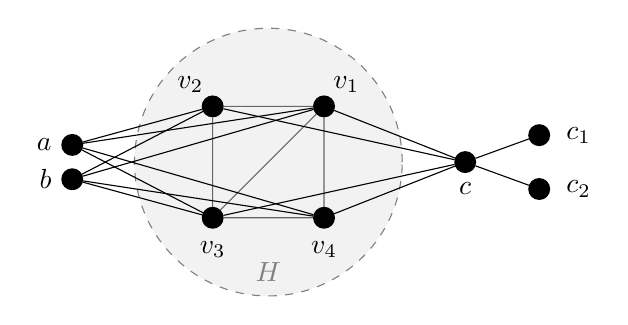
\begin{tikzpicture}					
		%---------- H CORE  --------------- 		
		\fill[lgray, dashed] (0,0) circle (1.7cm);
		
		\node [std](v1) at (45:1cm) {};
		\path (v1) ++(45:4 mm) node (x1L) {$v_1$};
		\node [std](v2) at (135:1cm){};
		\path (v2) ++(135:4 mm) node (x2L) {$v_2$};
		\node [std](v3) at (225:1cm) {};
		\path (v3) ++(270:4 mm) node (x3L) {$v_3$};
		\node [std](v4) at (315:1cm){};
		\path (v4) ++(270:4 mm) node (x4L) {$v_4$};
		\draw[mgray](v1)--(v2)--(v3)--(v4)--(v1)--(v3);
		
		\draw[gray, dashed] (0,0) circle (1.7cm);
		\node (H) at (0,-1.4) [color=gray](L){$H$};	
		%--------- A B C ----------------------					
		
		\node [std](a) at (175:25mm)[label=left:$a$]  {};			
		\node [std](b) at (185:25mm)[label=left:$b$]  {};	
		
		
		\node [std](c) at (0:25mm)[label=below:$c$]  {};	
		
		\foreach \i in {1,2,3,4}
		{\draw(a)--(v\i)--(b);
			\draw(c)--(v\i);}
		
		\foreach \i / \j in {1/20, 2/-20}
		{ \path (c) ++(\j:10 mm) node (c\i) [std] {};
			\path (c\i) ++(0:5 mm) node (cL\i)  {$c_{\i}$};	
			\draw(c)--(c\i);
		}
		
	\end{tikzpicture}
	\caption{The graph $G$ constructed from $H$ from \cite{CHH10}.}%
	\label{fig:gprConst}%
\end{figure}
%~~~~~~~~~~~~~~~~~~~~~~~~~FIG END~~~~~~~~~~~~~~~~~~~~~~


From the pendant vertices, $c$ is in every $\gamma$-set of $G$; however, as
$a$ and $b$ remain undominated, $\{c\}$ is not itself a $\gamma$-set. Thus,
$\gpr(G) \geq\gamma(G) \geq2$ (likewise $\gamma_{c}(G) \geq\gt(G) \geq
\gamma(G) \geq2$). It follows that for each $v_{i}\in V(H)$, the set
$S_{i}=\{c,v_{i}\}$ is a $\gamma$-set. Since $\ir(G) \leq2 = \gamma(G) \leq2
\ir(G)-1$, it follows that $S_{i}$ is an $\ir$-set. Moreover, since $cv_{i}
\in E(G)$, each $S_{i}$ is also a $\gpr$-set, a $\gt$-set, and $\gamma_{c}%
$-set. Since neither $\{c,a\}$ nor $\{ c,b\}$ is dominating, the collection
$\{S_{i}: 1 \leq i \leq n\}$ consists of all the $\ir$, $\gamma$, $\gt$,
$\gpr$, $\gamma_{c}$-sets of $G$.

%-----	GAMMA + ID GRAPH PROOF ---

\section{The $\gid$-Graph}

\label{subsec:GIDExist}

A popular variation on domination is the topic of identifying codes. A vertex
set $S$ is an \emph{identifying code} (ID-code) of a graph $G$ if for each $v \in V$, the
closed neighbourhood of $v$ and $S$ have a unique, nonempty intersection. The
\emph{intersection set} of a vertex $v$ with respect to a vertex subset $S$ is
the set $I_{S}(v) = N[v]\cap S$. Thus, $S$ is an identifying code of $G$ if
all of its intersection sets are unique and nonempty.  The
cardinality of a minimum ID-code is denoted $\gid(G)$, and an ID-code with
cardinality $\gid(G)$ is called an $\gid$-\emph{set}. If $\gid(G)$ is finite,
$G$ is said to be \emph{identifiable} (or \emph{distinguishable}); otherwise,
$G$ is not identifiable, and $\gid(G)$ is defined to be $\gid(G)=\infty$. 

Originally introduced by Karpovsky et al. in 1998 \cite{KCL98}, ID-codes were
proposed as a model for the positioning of fault-detection units on
multiprocessor systems (for additional references, see Lobstein's extensive
bibliography \cite{Biblio}). Consider now the problem of migrating the
detecting units from one configuration to another, such that only one
detecting unit can be moved at time to an adjacent processor, and at each step
the configuration remains an ID-code. When given a certain starting
configuration, what other configurations are reachable under these conditions?
How many steps are required to move between them? Are there multiple routes
from start to destination, or are we stuck with a single path? To aid in
addressing this family of questions, we define the $\gid$-\emph{graph of a
	graph $G$}, $G(\gid)=(V(\gid),E(\gid))$, similarly to the $\gamma$-graph, but
where the vertices now correspond to the $\gid$-sets in $G$ instead.

As a first result, we extend Theorem \ref{thm:sl:gammaGraph} to
$\gid$-graphs. The construction and proof are similar; however, in
consideration of the additional identification requirements, multiple copies
of the graph $\mathcal{C} = C_{4}\circleddash K_{1}$, the \emph{depleted
	corona of $C_{4}$}, in Figure \ref{fig:gidHand} are used to force certain
vertices into the $\gid$-set. Given any graph $G^{\prime}$, we construct a new
graph $G$ by adding an edge between $x_{1} \in V(\mathcal{C})$ and some $v\in
V(G^{\prime})$; we say $\mathcal{C}$ is \emph{attached to $G^{\prime}$ at $v$}.

%~~~~~~~~~~~~~~~~~~~~~~~~~FIG START~~~~~~~~~~~~~~~~~~~~~~
\begin{figure}[tbh]
	\centering
	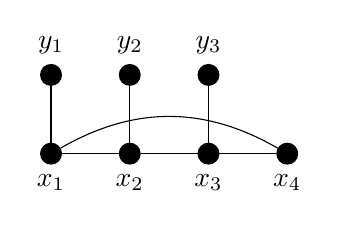
\begin{tikzpicture}				
		
		%-----------X PATH ------------------								
		\foreach \i/\x in {1/1.5, 2/2.5,3/3.5,4/4.5}
		\node [std](x\i) at (\x,1.5)[label=below:$x_\i$] {};	
		
		\draw(x1)--(x2)--(x3)--(x4);		
		
		%---------- Y LEAVES  --------------- 									
		\foreach \i/\x in {1/1.5, 2/2.5,3/3.5}
		\node [std](y\i) at (\x,2.5)[label=above:$y_\i$] {};							
		
		\foreach \i/\x in {1/1.5, 2/2.5,3/3.5}
		\draw (y\i)--(x\i);
		
		\draw(x1) to [out=30,in=150](x4);								
		
	\end{tikzpicture}
	\caption{The graph $\mathbf{\mathcal{C}}$ in Lemmas \ref{lem:C} and
		\ref{lem:gidHand}.}%
	\label{fig:gidHand}%
\end{figure}
%~~~~~~~~~~~~~~~~~~~~~~~~~FIG END~~~~~~~~~~~~~~~~~~~~~~


\begin{lemma}
	\label{lem:C}  The vertex set $X=\{x_{1},x_{2},x_{3}\}$ is the unique
	$\gid$-set of $\mathcal{C}$.
\end{lemma}

%### Proof Start


\begin{proof}
	Suppose that $\mathcal{C}$ has a $\gid$-set $S$. Since the vertices in
	$Y=\{y_{1},y_{2},y_{3}\}$ are all pendant vertices in $\mathcal{C}$, for each
	$1 \leq i \leq3$, either $x_{i}$ or $y_{i}$ is in $S$. Since $X$ is
	identifying, it follows that $\gid(\mathcal{C}) = 3$ and that $X$ is a
	$\gid$-set of $\mathcal{C}$.
	
	Notice that since $|S|=3$ and each $y_{i}$ is pendant, $S\subseteq X\cup Y$
	and $x_{4}\notin S$. To dominate $x_{4}$, either $x_{1}$ or $x_{3}$ is in $S$.
	Without loss of generality, say $x_{1} \in S$. To show uniqueness, we need
	only verify that the sets $S_{2}=\{x_{1},y_{2},x_{3}\}$, $S_{3}=\{x_{1}%
	,x_{2},y_{3}\}$ and $S_{2,3}=\{x_{1},y_{2},y_{3}\}$ are not identifying. For
	$S_{2}$, $I_{S_{2}}(x_{3})= I_{S_{2}}(y_{3})=\{x_{3}\}$ and is therefore not
	identifying. Likewise for $S_{2,3}$, $I_{S_{2,3}}(x_{3})= I_{S_{2,3}}%
	(y_{3})=\{y_{3}\}$. Finally for $S_{3}$, $I_{S_{3}}(x_{4})= I_{S_{3}}%
	(y_{1})=\{x_{1}\}$. It follows that $S=X =\{x_{1},x_{2},x_{3}\}$ is the unique
	$\gid$-set of $\mathcal{C}$.
\end{proof}

%### Proof End


\begin{lemma}
	\label{lem:gidHand}  Let $G^{\prime}$ be any graph, and construct $G$ by
	attaching $\mathcal{C}$ to $G^{\prime}$ at some $v\in V(G^{\prime})$. If $S$
	is any $\gid$-set of $G$, then $\{x_{1},x_{2},x_{3}\} \subseteq S$. Moreover,
	if $S^{\prime}$ is a $\gid$-set of $G^{\prime}$, then $S^{\prime}\cup
	\{x_{1},x_{2},x_{3}\}$ is identifying in $G$.
\end{lemma}

%### Proof Start


\begin{proof}
	Let $V(G^{\prime}) = \{v_{1},v_{2},\dots,v_{n}\}$, and suppose that $G$ was
	constructed by attaching $\mathcal{C}$ to $G^{\prime}$ at $v_{n}$. Suppose
	that $G$ has an $\gid$-set $S$. Regardless of whether $v_{n} $ is in $S$ or
	not, each vertex of $Y=\{y_{1},y_{2},y_{3}\}$ remains pendant and so for each
	$1 \leq i \leq3$, either $x_{i}$ or $y_{i}$ is in $S$. Using the same
	arguments as in Lemma \ref{lem:C}, $\{x_{1},x_{2},x_{3}\} \subseteq S$.
	
	Now suppose that $S^{\prime}$ is a $\gid$-set of $G^{\prime}$ and consider
	$S=S^{\prime}\cup\{x_{1},x_{2},x_{3}\}$ in $G$. Since $S^{\prime}$ is
	identifying, for each $v_{i} \in V(G^{\prime})$, the intersection set
	$I_{S^{\prime}}(v_{i})$ in $G^{\prime}$ is unique. In $G$, all intersection
	sets of $v_{1}, v_{2}, \dots, v_{n-1}$ remain the same. The intersection set
	of $v_{n}$ becomes $I_{S}(v_{n}) = I_{S^{\prime}}(v_{n}) \cup\{x_{1}\} \neq
	I_{s}(y_{1})$. From the first portion of this lemma, the sets $I_{S}(x_{i})$
	for $1 \leq i \leq4$ are also unique. It follows that $S$ is identifying in
	$G$.
\end{proof}

%### Proof End


Notice that the converse of the second portion of Lemma \ref{lem:gidHand} does
not hold. For a counterexample, consider the graph $G$ in Figure
\ref{fig:leCE} constructed by attaching $\mathcal{C}$ to a copy of $C_{4}$
with $V(C_{4}) =\{v_{1},v_{2},v_{3},v_{4}\}$. Although $\{v_{1},v_{3}%
,x_{1},x_{2},x_{3}\}$ is a $\gid$-set of $G$, $\{v_{1},v_{3}\}$ is not a
$\gid$-set of $C_{4}$.



%~~~~~~~~~~~~~~~~~~~~~~~~~FIG START~~~~~~~~~~~~~~~~~~~~~~
\begin{figure}[H]
	\centering
	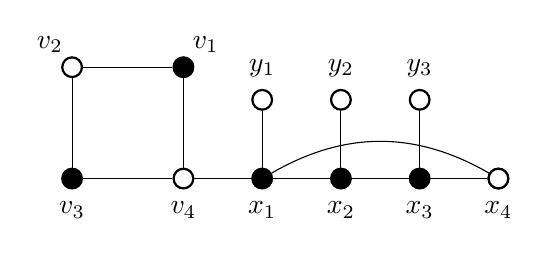
\begin{tikzpicture}					
		%---------- H CORE  --------------- 								
		\node [std](v1) at (45:1cm) {};
		\path (v1) ++(45:4 mm) node (x1L) {$v_1$};
		\node [wstd](v2) at (135:1cm){};
		\path (v2) ++(135:4 mm) node (x2L) {$v_2$};
		\node [std](v3) at (225:1cm) {};
		\path (v3) ++(270:4 mm) node (x3L) {$v_3$};
		\node [wstd](v4) at (315:1cm){};
		\path (v4) ++(270:4 mm) node (x4L) {$v_4$};
		\draw(v1)--(v2)--(v3)--(v4)--(v1);								
		
		%---------- X ------------------					
		\foreach \label/\rad in {1/10,2/20,3/30,4/40}
		\path (v4) ++(0:\rad mm) node (x\label) [std]  {};
		\draw(v4)--(x4);
		
		\foreach \i in {1, 2,3,4}
		\path (x\i) ++(-90:4 mm) node (xL\i) {$x_{\i}$};				
		
		%-----------Y -------------------					
		\foreach \i/\x in {1,2,3}
		{	\path (x\i) ++(90:10 mm) node (y\i) [wstd]  {};
			\draw (y\i)--(x\i);			
			\path (y\i) ++(90:4 mm) node (yL\i) {$y_{\i}$};	
		}
		
		\draw(x1) to [out=30,in=150](x4);			
		\node [wstd](x4w) at (x4){};										
		
	\end{tikzpicture}
	\caption{Counterexample to the converse of Lemma \ref{lem:gidHand}.}%
	\label{fig:leCE}%
\end{figure}
%~~~~~~~~~~~~~~~~~~~~~~~~~FIG END~~~~~~~~~~~~~~~~~~~~~~


\begin{theorem}
	\label{thm:gamma-ID}  Every graph $H$ is the $\gid$-graph of some graph.
\end{theorem}

%### Proof START


\begin{proof}
	Let $H = (V(H),E(H))$ be any nonempty graph with $V(H) = \{v_{1},v_{2}%
	,\dots,v_{n}\}$. We construct a new graph $G$ such that $G(\gid) \cong H$.
	
	\noindent\underline{Construction:} Begin with a copy of $H$ and for each
	$v_{i} \in V(H)$, attach two copies of the graph $\mathcal{C}$ from Figure
	\ref{fig:gidHand} to $H$ at $v_{i}$, labelled as $\mathcal{C}_{i}$ and
	$\mathcal{C}_{i}^{*}$ with 	
	\begin{align*}
	V(\mathcal{C}_{i}) = \{x_{i,1},x_{i,2},x_{i,3},x_{i,4}, y_{i,1}, y_{i,2}, y_{i,3}\}, \text{ and } 
	V(\mathcal{C}_{i}^{*}) = \{x_{i,1}^{*},x_{i,2}^{*},x_{i,3}^{*}, x_{i,4}^{*}, y_{i,1}^{*}, y_{i,2}^{*},
	y_{i,3}^{*}\}. 
	\end{align*}
	\noindent Now, add vertices $a$ and $b$ so that $av_{i} \in E(G)$ and
	$bv_{i} \in E(G)$ for all $i=1,2,\dots, n$. Finally, attach two more copies of
	$\mathcal{C}$, $\mathcal{C}_{a}$ and $\mathcal{C}_{b}$, at $a$ and $b$,
	respectively (see Figure \ref{fig:gidConst}).
	
	\noindent Consider the vertex set,
	\begin{align*}
		X = \left( \bigcup\limits_{\substack{1 \leq j \leq n \\1 \leq k \leq3}}
		\{x_{j,k}, x_{j,k}^{*}\}\right)  \cup\left( \bigcup\limits_{1\leq k \leq3}
		\{x_{a,k},x_{b,k}\}\right) .
	\end{align*}
	In particular, notice that $X$ consists of all the vertices within the various
	$\mathcal{C}$ graphs that Lemma \ref{lem:gidHand} demonstrates are in every
	$\gid$-set of $G$.
	
	%~~~~~~~~~~~~~~~~~~~~~~~~~FIG START~~~~~~~~~~~~~~~~~~~~~~
	\begin{figure} 
		\centering %\scalebox{0.85}{
			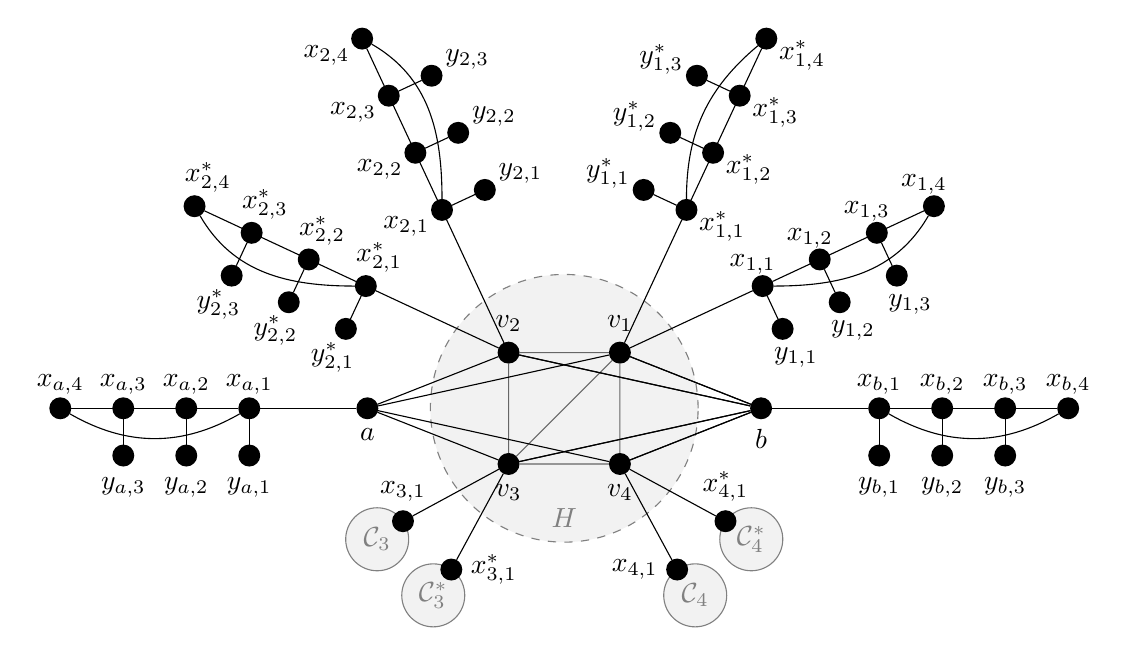
\begin{tikzpicture}				
				%---------- H CORE  --------------- 		
				\fill[lgray, dashed] (0,0) circle (1.7cm);
				
				\node [std](v1) at (45:1cm)[label=above:$v_1$] {};
				\node [std](v2) at (135:1cm)[label=above:$v_2$] {};
				\node [std](v3) at (225:1cm)[label=below:$v_3$] {};
				\node [std](v4) at (315:1cm)[label=below:$v_4$] {};
				\draw[mgray](v1)--(v2)--(v3)--(v4)--(v1)--(v3);
				
				\draw[gray, dashed] (0,0) circle (1.7cm);
				\node (H) at (0,-1.4) [color=gray](L){$H$};			
				
				%---------- X Stems  --------------- 									
				\node (x31) at (215:25mm) [label=above:$x_{3,1}$] {};
				\node (x41) at (305:25mm) [label=left:$x_{4,1}$] {};
				
				\draw(v3)--(x31);
				\draw(v4)--(x41);
				%---------- X* Stems  --------------- 									
				\node (x31*) at (235:25mm)[label=right:$x_{3,1}^*$] {};
				\node (x41*) at (325:25mm) [label=above:$x_{4,1}^*$]{};	
				\draw(v3)--(x31*);
				\draw(v4)--(x41*);
				
				%-----------X1 PATHS ------------------
				\path (v1) ++(25:20 mm) node (x11) [std]  {};
				\draw(v1)--(x11);
				
				\foreach \label/\rad in {2/8,3/16,4/24}
				\path (x11) ++(25:\rad mm) node (x1\label) [std]  {};
				\draw(x11)--(x14);
				
				\foreach \x/\i in {1/2, 2/2,3/2,4/2}
				\path (x1\x) ++(115:3 mm) node (x1L\x) {$x_{1,\x}$};										
				
				\foreach \x/\y in {1/1, 2/2, 3/3}
				\path (x1\x) ++(-65:6mm) node (y1\y) [std]  {};
				\foreach \x/\y in {1/1, 2/2,3/3}
				\draw(x1\x)--(y1\y);	
				
				\foreach \y/\i in {1/2, 2/2,3/2}
				\path (y1\y) ++(-65:4 mm) node (y1L\y) {$y_{1,\y}$};								
				
				\draw(x11) to [out=0,in=240](x14);	
				
				%-----------X1* PATHS ------------------
				\path (v1) ++(65:20 mm) node (x11*) [std]  {};
				\draw(v1)--(x11*);
				
				\foreach \label/\rad in {2/8,3/16,4/24}
				\path (x11*) ++(65:\rad mm) node (x1\label*) [std]  {};
				\draw(x11*)--(x14*);							
				
				\foreach \x/\i in {1/2, 2/2,3/2,4/2}
				\path (x1\x*) ++(-25:5 mm) node (x1L\x*) {$x_{1,\x}^*$};									
				
				\foreach \x/\y in {1/1, 2/2, 3/3}
				\path (x1\x*) ++(155:6mm) node (y1\y*) [std]  {};
				\foreach \x/\y in {1/1, 2/2,3/3}
				\draw(x1\x*)--(y1\y*);				
				
				\foreach \y/\i in {1/2, 2/2,3/2}
				\path (y1\y*) ++(155:5 mm) node (y1L\y*) {$y_{1,\y}^*$};										
				
				\draw(x11*) to [out=90,in=220](x14*);
				%-----------X2 PATHS ------------------
				\path (v2) ++(115:20 mm) node (x21) [std]  {};
				\draw(v2)--(x21);
				
				\foreach \label/\rad in {2/8,3/16,4/24}
				\path (x21) ++(115:\rad mm) node (x2\label) [std]  {};
				\draw(x21)--(x24);
				
				\foreach \x/\i in {1/2, 2/2,3/2,4/2}
				\path (x2\x) ++(205:5 mm) node (x2L\x) {$x_{2,\x}$};										
				
				\foreach \x/\y in {1/1, 2/2, 3/3}
				\path (x2\x) ++(25:6mm) node (y2\y) [std]  {};
				\foreach \x/\y in {1/1, 2/2,3/3}
				\draw(x2\x)--(y2\y);	
				
				\foreach \y/\i in {1/2, 2/2,3/2}
				\path (y2\y) ++(25:5 mm) node (y2L\y) {$y_{2,\y}$};								
				
				\draw(x21) to [out=90,in=330](x24);	
				
				%-----------X2* PATHS ------------------
				\path (v2) ++(155:20 mm) node (x21*) [std]  {};
				\draw(v2)--(x21*);
				
				\foreach \label/\rad in {2/8,3/16,4/24}
				\path (x21*) ++(155:\rad mm) node (x2\label*) [std]  {};
				\draw(x21*)--(x24*);							
				
				\foreach \x/\i in {1/2, 2/2,3/2,4/2}
				\path (x2\x*) ++(65:4 mm) node (x2L\x*) {$x_{2,\x}^*$};									
				
				\foreach \x/\y in {1/1, 2/2, 3/3}
				\path (x2\x*) ++(245:6mm) node (y2\y*) [std]  {};
				\foreach \x/\y in {1/1, 2/2,3/3}
				\draw(x2\x*)--(y2\y*);				
				
				\foreach \y/\i in {1/2, 2/2,3/2}
				\path (y2\y*) ++(245:4 mm) node (y2L\y*) {$y_{2,\y}^*$};										
				
				\draw(x21*) to [out=180,in=300](x24*);	
				
				%--------- A ----------------------			
				\node [std](a) at (180:25mm)[label=below:$a$]  {};			
				
				\foreach \i in {1,2,3,4}
				\draw(a)--(v\i);
				
				\path (a) ++(180:15 mm) node (xa1) [std]  {};
				\draw(a)--(xa1);
				
				\foreach \label/\rad in {2/8,3/16,4/24}
				\path (xa1) ++(180:\rad mm) node (xa\label) [std]  {};
				\draw(xa1)--(xa4);
				
				\foreach \x in {1, 2,3,4}
				\path (xa\x) ++(90:3 mm) node (xaL\x) {$x_{a,\x}$};										
				
				\foreach \x/\y in {1/1, 2/2, 3/3}
				\path (xa\x) ++(270:6mm) node (ya\y) [std]  {};
				\foreach \x/\y in {1/1, 2/2,3/3}
				\draw(xa\x)--(ya\y);	
				
				\foreach \y/\i in {1/2, 2/2,3/2}
				\path (ya\y) ++(270:4 mm) node (yaL\y) {$y_{a,\y}$};								
				
				\draw(xa1) to [out=210,in=-30](xa4);	
				
				%--------- B ----------------------						
				\node [std](b) at (0:25mm)[label=below:$b$]  {};					
				
				\foreach \i in {1,2,3,4}
				\draw(b)--(v\i);
				
				\draw(b)--(v1);
				\draw(b)--(v2);
				\draw(b)--(v3);
				\draw(b)--(v4);
				
				\path (b) ++(0:15 mm) node (xb1) [std]  {};
				\draw(b)--(xb1);
				
				\foreach \label/\rad in {2/8,3/16,4/24}
				\path (xb1) ++(0:\rad mm) node (xb\label) [std]  {};
				\draw(xb1)--(xb4);
				
				\foreach \x in {1, 2,3,4}
				\path (xb\x) ++(90:3 mm) node (xbL\x) {$x_{b,\x}$};										
				
				\foreach \x/\y in {1/1, 2/2, 3/3}
				\path (xb\x) ++(270:6mm) node (yb\y) [std]  {};
				\foreach \x/\y in {1/1, 2/2,3/3}
				\draw(xb\x)--(yb\y);	
				
				\foreach \y/\i in {1/2, 2/2,3/2}
				\path (yb\y) ++(270:4 mm) node (ybL\y) {$y_{b,\y}$};								
				
				\draw(xb1) to [out=-30,in=210](xb4);														
				
				% ----------- BLOBS ---------------------
				% Z3 - Blob
				\path (x31) ++(215:4 mm) node (x31C){};
				\fill[lgray] (x31C) circle (4mm);
				\draw[gray] (x31C) circle (4mm){};
				\node[std] at (x31){};
				\node at  (x31C) [color=gray]{$\mathcal{C}_3$};	
				
				% Z3* - Blob	
				\path (x31*) ++(235:4 mm) node (x31C*){};
				\fill[lgray] (x31C*) circle (4mm);
				\draw[gray] (x31C*) circle (4mm){};
				\node[std] at (x31*){};
				\node at  (x31C*) [color=gray]{$\mathcal{C}_3^*$};							
				
				% Z4 - Blob
				\path (x41) ++(305:4 mm) node (x41C){};
				\fill[lgray] (x41C) circle (4mm);
				\draw[gray] (x41C) circle (4mm){};
				\node[std] at (x41){};
				\node at  (x41C)[color=gray]{$\mathcal{C}_4$};
				
				% Z4* - Blob
				\path (x41*) ++(325:4 mm) node (x41C*){};
				\fill[lgray] (x41C*) circle (4mm);
				\draw[gray] (x41C*) circle (4mm){};
				\node[std] at (x41*){};
				\node at  (x41C*)[color=gray]{$\mathcal{C}_4^*$};
				
			\end{tikzpicture} %}
		\caption{The graph $G$ constructed from $H$ in Theorem \ref{thm:gamma-ID}. }%
		\label{fig:gidConst}% 
	\end{figure}
	%~~~~~~~~~~~~~~~~~~~~~~~~~FIG END~~~~~~~~~~~~~~~~~~~~~~
	
	
	We first show that for each $1 \leq i \leq n$, the vertex set $S_{i} =
	\{v_{i}\}\cup X$ is a $\gid$-set of $G$. From the construction of $G$, it is
	clear that $S_{i}$ dominates $G$. Furthermore, from Lemma \ref{lem:gidHand},
	we know that each vertex within a $\mathcal{C}$ subgraph is identified by
	$S_{i}$. For vertices within $H$, the identifying set $I_{S_{i}}(v_{j})$ of
	the vertex $v_{j}$ contains the unique pair $\{x_{j,1},x_{j,1}^{*}\}$,
	ensuring that each $v_{j}$ is identified in $S_{i}$. Finally, $a$ and $b$ also
	have the unique identifying sets $I_{S_{i}}(a)=\{x_{a,1}, v_{i}\}$ and
	$I_{S_{i}}(b) = \{x_{b,1}, v_{i}\}$, respectively. It follows that $S_{i}$ is
	identifying and dominating in $G$.
	
	We now show that $S_{i}$ is a $\gid$-set. Notice that there are $2n+6$ pendant
	vertices in $G$, and so $\gamma(G) \geq2n+6$. Indeed, it is easy to see that
	$X=S_{i}-\{v_{i}\}$ is dominating in $G$, so $\gamma(G) = 2n+6$. Moreover,
	$\gid(G) \geq\gamma(G) = 2n+6$. Again, by Lemma \ref{lem:gidHand}, we know
	that any $\gid$-set of $G$ contains all of $X$; however $X$ is not identifying
	as $I_{X}(a) = \{x_{a,1}\} = I_{X}(y_{a,1})$, and so, $\gid(G) \geq(2n+6)+1$.
	Since $|S_{i}|=2n+7$ and $S_{i}$ is identifying, it follows that $S_{i}$ is a
	$\gid$-set for all $\leqn$.
	
	Let $\mathcal{S}_{\gid}=\{S_{1},S_{2},\dots,S_{n}\}$. We claim that
	$\mathcal{S}_{\gid}$ is the collection of all $\gid$-sets of $G$. Since we
	have already established that $\gid(G)=2n+7$ and that in every $\gid$-set,
	$2n+6$ of the vertices are from $X$, every $\gid$-set of $G$ can viewed as
	\textquotedblleft$X$-plus-one\textquotedblright. However, there is no single
	vertex $w\in V(G)-V(H)$ such that $X\cup\{w\}$ identifies both pairs
	$\{a,y_{a,1}\}$ and $\{b,y_{b,1}\}$. The set $S_{a}=\{a\}\cup X$ with $|S_{a}|=2n+7$
	has $I_{S_{a}}(b)=\{x_{b,1}\}=I_{S_{a}}(y_{b,1})$ and is therefore not
	identifying. Similarly, $S_{b}=\{b\}\cup X$ is not identifying. Thus,
	$\mathcal{S}_{\gid}$ is the collection of all $\gid$-sets.
	
	Consider now $G(\gid) = (V(\ggid),E(\ggid))$. By the above arguments,
	$V(\ggid)$ $= \{v_{1}^{\prime},v_{2}^{\prime},\dots,v_{n}^{\prime}\}$, where
	the vertex $v_{i}^{\prime}$ corresponds to the set $S_{i} \in\mathcal{S}%
	_{\gid}$ for each $\leqn$. Since $v_{i}^{\prime}$ and $v_{j}^{\prime}$ in
	$V(\ggid)$ are adjacent in $\ggid$ if and only if there exist $w_{i}\in S_{i}$
	and $w_{j} \in S_{j}$ with $w_{i}w_{j}\in E(G)$ such that $S_{i} = (S_{j}
	-\{w_{j}\}) \cup\{w_{i}\}$ and $S_{i}$ and $S_{j}$ differ at exactly one
	vertex (that is, $v_{i}$ versus $v_{j}$), it follows that $v_{i}^{\prime}%
	v_{j}^{\prime}\in E(\gid)$ if and only if $v_{i}v_{j} \in E(G)$. Therefore,
	$\ggid \cong H$ as required.
\end{proof}

%### Proof End


In the construction of the graph $G$ in the proof of Theorem
\ref{thm:gamma-ID}, if instead of attaching only two copies of the graph
$\mathcal{C}$ to each vertex of the graph $H$, we attached three or more
copies, the same $\gid$-graph $H$ is obtained. This leads immediately to the
following corollary.

\begin{coro}
	Every graph $H$ is the $\gid$-graph of infinitely many graphs.
\end{coro}

%----------------------SUBSEC: Locating ----------------------------------------------------
\section{The $\gamma_{L}$ and $\gamma_{t}^{L}$-Graphs}

Introduced by Slater in 1988 \cite{Slater87, Slater88}, a \emph{locating-dominating set}
$S$ of graph $G=(V,E)$ is a dominating set such that for each $v\in V-S$, the
set $N[v] \cap S$ is unique. In contrast to identifying codes,
locating-dominating sets do not require that the vertices of the dominating
set have unique neighbourhood intersection with the dominating set itself. The
minimum cardinality of a locating-dominating set, denoted by $\gamma_{L}(G)$,
is the \emph{locating-domination number} of a graph $G$. A \emph{$\gamma_{L}%
	$-set} of a graph is a minimum locating-dominating vertex subset. Since all
identifying codes are also locating-dominating sets, it follows that
$\gamma_{L} \leq\gid$ for all graphs. We reuse the notation of the
intersection set of a vertex $v$ and set $S$ from ID-codes; however, for
locating-dominating sets, the sets $I_{S}(v)$ need only be unique for $v\notin S$.

We define the \emph{$\gamma_{L}$-graph of a graph $G$}, $G(\gamma
_{L})=(V(\gamma_{L}),E(\gamma_{L}))$, to the be graph where the vertex set
$V(\gamma_{L})$ is the collection of $\gamma_{L}$-sets of $G$. As with the
$\gamma$-graph, $u,w \in V(\gamma_{L})$ associated with $\gamma_{L}$-sets
$S_{u}$ and $S_{w}$ are adjacent in $G(\gamma_{L})$ if and only if there exist
$v_{u} \in S_{u}$ and $v_{w} \in S_{w}$ with $v_{u}v_{w}\in E(G)$, such that
$S_{u} = (S_{w} - \{v_{w}\}) \cup\{v_{u}\}$.

Given the similarities between ID-codes and locating-dominating sets, it is
not surprising that a similar result to Theorem \ref{thm:gamma-ID} exists for
$\gamma_{L}$-graphs.

\begin{theorem}
	\label{thm:gammaL} Every graph $H$ is the $\gamma_{L}$-graph of infinitely
	many graphs.
\end{theorem}

Since $\mathcal{C}$ does not have a unique $\gamma_{L}$-set (for example,
$\{x_{1},x_{2},x_{3}\}$ and $\{x_{1},x_{2},y_{3}\}$ are $\gamma_{L}$-sets), we
cannot use it in the construction to prove Theorem \ref{thm:gammaL}. Instead,
we use the very similar \emph{Bull graph}, $\bull$, as pictured in Figure
\ref{fig:gLhand}. Notice that $S=\{x_{1},x_{2}\}$ is a $\gamma_{L}$-set in
$\bull$. Moreover, since $S_{1}=\{x_{1}, y_{2}\}$ and $S_{2}=\{y_{1},x_{2}\}$
give $I_{S_{1}}(y_{1})=\{x_{1}\}=I_{S_{1}}(x_{3})$, and $I_{S_{2}}%
(y_{2})=\{x_{2}\}=I_{S_{2}}(x_{3})$, $S$ is the only $\gamma_{L}$-set of
$\bull$. The proof to Theorem \ref{thm:gammaL} then proceeds identically to
that of Theorem \ref{thm:gamma-ID}, substituting the use of $\bull$ for
$\mathcal{C}$.



%~~~~~~~~~~~~~~~~~~~~~~~~~FIG START~~~~~~~~~~~~~~~~~~~~~~
\begin{figure}[H]
	\centering
	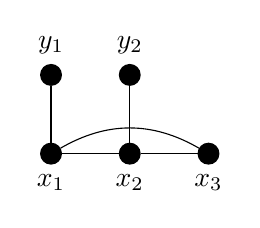
\begin{tikzpicture}				
		
		%-----------X PATH ------------------								
		\foreach \i/\x in {1/1.5, 2/2.5,3/3.5}
		\node [std](x\i) at (\x,1.5)[label=below:$x_\i$] {};	
		
		\draw(x1)--(x2)--(x3);		
		
		%---------- Y LEAVES  --------------- 									
		\foreach \i/\x in {1/1.5, 2/2.5}
		\node [std](y\i) at (\x,2.5)[label=above:$y_\i$] {};							
		
		\foreach \i/\x in {1/1.5, 2/2.5}
		\draw (y\i)--(x\i);
		
		\draw(x1) to [out=30,in=150](x3);								
		
	\end{tikzpicture}
	\caption{The Bull graph $\bull$ used in the construction of Theorem
		\ref{thm:gammaL}.}%
	\label{fig:gLhand}%
\end{figure}
%~~~~~~~~~~~~~~~~~~~~~~~~~FIG END~~~~~~~~~~~~~~~~~~~~~~

A variant of locating-dominating sets, a vertex subset $S$ is a
\emph{locating-total dominating set} (LTDS) of a graph $G$ if $S$ a
locating-dominating set and if each vertex in $V(G)$ is adjacent to some
vertex in $S$. The \emph{locating-total domination number} $\gamma_{t}^{L}(G)$
is the minimum cardinality of a LTDS \cite{HHH06}. We define the $\gamma
_{t}^{L}$-graph of a graph $G$ analogously to the $\gamma_{L}$-graph. Since in
the construction of Theorem \ref{thm:gammaL}, there were no independent
vertices in the $\gamma_{L}$-sets, the following corollary is immediate.

\begin{coro}
	Any graph $H$ is the $\gamma_{t}^{L}$-graph of infinitely many graphs.
\end{coro}

%----------------------SUBSEC: BIG GAMMA  ----------------------------------------


\section{The $\Gamma$-Graph}

The next domination parameter we examine is $\Gamma(G)$, the
\emph{upper domination number} of a graph $G$, defined to be the cardinality
of a largest minimal dominating set. The \emph{$\Gamma$-graph of a graph $G$}
and its associated parameters are defined analogously to $G(\gamma)$. Once
again, this variation requires the use of a new gadget: the graph
$\mathcal{Z}$ in Figure \ref{fig:Z}.

%~~~~~~~~~~~~~~~~~~~~~~~~~FIG START~~~~~~~~~~~~~~~~~~~~~~
\begin{figure}[H] 
	\centering
	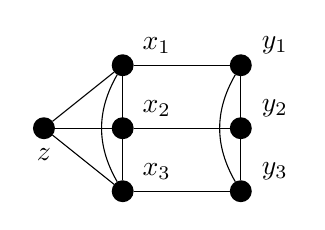
\begin{tikzpicture}								
		
		%---------- Add on------------------
		\node [std](z) at (0,0)[label=below:$z$]  {};						
		
		\path (z) ++(0:10 mm) node (x2) [std] {};
		\draw(z)--(x2);	
		
		\foreach \i / \j in {1/90, 3/-90}
		{ \path (x2) ++(\j:8 mm) node (x\i) [std] {};
			\draw(z)--(x\i);
		}							
		
		\draw(x1)--(x3);	
		\draw(x1) to [out=-120,in=120](x3);		
		
		\foreach \i / \j  in {1/30, 2/30, 3/30}
		{
			\path (x\i) ++(0:15 mm) node (y\i) [std] {};
			\path (y\i) ++(\j:5 mm) node (yL\i)  {$y_{\i}$};
			\path (x\i) ++(\j:5 mm) node (xL\i)  {$x_{\i}$};		
			\draw(x\i)--(y\i);									
		}	
		
		\draw(y1)--(y3);	
		\draw(y1) to [out=-120,in=120](y3);		
		
	\end{tikzpicture} 
	\caption{The graph $\mathcal{Z}$ used in Theorem \ref{thm:bigGamma}.}%
	\label{fig:Z}%
\end{figure}
%~~~~~~~~~~~~~~~~~~~~~~~~~FIG END~~~~~~~~~~~~~~~~~~~~~~


\begin{theorem}
	\label{thm:bigGamma} Every graph $H$ is the $\Gamma$-graph of infinitely many graphs.
\end{theorem}

%## START PROOF


\begin{proof}
	\underline{Construction:} The construction of a graph $G$ with $G(\Gamma
	)\cong H$ is similar to the previous results. Begin with a copy of the graph
	$H$ with $V(H)=\{v_{1}, v_{2}, \dots, v_{n}\}$, and to each $v_{i}$, attach a
	copy of the graph $\mathcal{Z}$ in Figure \ref{fig:Z} labelled $\mathcal{Z}%
	_{i}$ with $V(Z_{i})=\{z_{i},x_{i,1},x_{i,2},x_{i,3}, y_{i,1}, y_{i,2},
	y_{i,3}\}$ at vertex $x_{i,1}$ to $v_{i}$. Attach a final copy of
	$\mathcal{Z}$ labelled $\mathcal{Z^{*}}$ ($V(\mathcal{Z}^{*})=\{z^{*}%
	,x_{1}^{*},x_{2}^{*},x_{3}^{*}, y_{1}^{*}, y_{2}^{*}, y_{3}^{*}\}$) by joining
	each $v_{i}$ to $z^{*}$.
	
	\noindent For reference, we define $X_{i} = \{x_{i,1}, x_{i,2}, x_{i,3}\}$,
	$Y_{i} = \{y_{i,1}, y_{i,2}, y_{i,3}\}$, $X^{*} = \{x_{1}^{*}, x_{2}^{*},
	x_{3}^{*}\}$, and $Y^{*} = \{y_{1}^{*}, y_{2}^{*}, y_{3}^{*}\}$.
	
	We claim that the $\Gamma$-sets of $G$ are $S_{1}, S_{2}, \dots, S_{n}$ where
	for each $1 \leq i \leq n$,
	\begin{align}
		S_{i} = \{v_{i}\} \cup\left( \bigcup_{1\leq j \leq n} X_{j} \right)  \cup
		Y^{*}.
	\end{align}
	
	
	%~~~~~~~~~~~~~~~~~~~~~~~~~FIG START~~~~~~~~~~~~~~~~~~~~~~
	\begin{figure}
		\centering \scalebox{0.9}{
			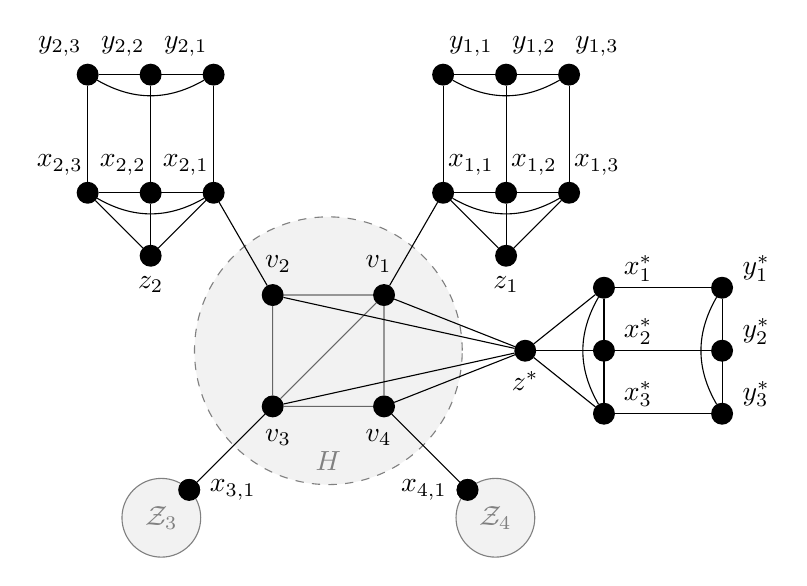
\begin{tikzpicture}					
				%---------- H CORE  --------------- 		
				\fill[lgray, dashed] (0,0) circle (1.7cm);
				
				\node [std](v1) at (45:1cm) {};
				\path (v1) ++(100:4 mm) node (x1L) {$v_1$};
				\node [std](v2) at (135:1cm){};
				\path (v2) ++(80:4 mm) node (x2L) {$v_2$};
				\node [std](v3) at (225:1cm) {};
				\path (v3) ++(280:4 mm) node (x3L) {$v_3$};
				\node [std](v4) at (315:1cm){};
				\path (v4) ++(260:4 mm) node (x4L) {$v_4$};
				\draw[mgray](v1)--(v2)--(v3)--(v4)--(v1)--(v3);
				
				\draw[gray, dashed] (0,0) circle (1.7cm);
				\node (H) at (0,-1.4) [color=gray](L){$H$};	
				%---------- X Stems  --------------- 		
				\path (v3) ++(225:15 mm) node (x31) [std][label=right:$x_{3,1}$] {};								
				\path (v4) ++(-45:15 mm) node (x41) [std][label=left:$x_{4,1}$] {};		
				
				\draw(v3)--(x31);
				\draw(v4)--(x41);
				
				% Z3 - Blob
				\path (x31) ++(225:5 mm) node (x31C){};
				\fill[lgray] (x31C) circle (5mm);
				\draw[gray] (x31C) circle (5mm){};
				\node[std] at (x31){};
				\node at  (x31C) [color=gray]{$\mathcal{Z}_3$};							
				
				% Z4 - Blob
				\path (x41) ++(-45:5 mm) node (x41C){};
				\fill[lgray] (x41C) circle (5mm);
				\draw[gray] (x41C) circle (5mm){};
				\node[std] at (x41){};
				\node at  (x41C)[color=gray]{$\mathcal{Z}_4$};
				%---------- Z1 ------------------
				
				\path (v1) ++(60:15 mm) node (x11) [std] {};
				
				\foreach \i / \j in {2/8, 3/16}
				{ \path (x11) ++(0: \j mm) node (x1\i) [std] {};
					\draw(x11)--(x1\i);								
				}
				
				\path (x12) ++(-90:8 mm) node (z1) [std] [label=below:$z_1$] {};
				\draw (x11)--(z1)--(x13);
				\draw(z1)--(x12);															
				
				\draw(x11)--(x13);	
				\draw(x11) to [out=-30,in=210](x13);		
				
				\foreach \i / \j  in {1/45, 2/45, 3/45}
				{
					\path (x1\i) ++(90:15 mm) node (y1\i) [std] {};
					\path (y1\i) ++(\j:5 mm) node (yL1\i)  {$y_{1,\i}$};							
					\draw(x1\i)--(y1\i);									
				}	
				
				\foreach \i / \j  in {1/45, 2/45, 3/45}	
				\path (x1\i) ++(\j:5 mm) node (xL1\i)  {$x_{1,\i}$};							
				
				\draw(y11)--(y13);	
				\draw(y11) to [out=-30,in=210](y13);						
				
				\draw(v1)--(x11);
				
				
				%---------- Z2 ------------------
				
				\path (v2) ++(120:15 mm) node (x21) [std] {};
				
				\foreach \i / \j in {2/8, 3/16}
				{ \path (x21) ++(180: \j mm) node (x2\i) [std] {};
					\draw(x21)--(x2\i);								
				}
				
				\path (x22) ++(-90:8 mm) node (z2) [std] [label=below:$z_2$] {};
				\draw (x21)--(z2)--(x23);
				\draw(z2)--(x22);															
				
				\draw(x21)--(x23);	
				\draw(x21) to [out=210,in=-30](x23);		
				
				\foreach \i / \j  in {1/135, 2/135, 3/135}
				{
					\path (x2\i) ++(90:15 mm) node (y2\i) [std] {};
					\path (y2\i) ++(\j:5 mm) node (yL2\i)  {$y_{2,\i}$};							
					\draw(x2\i)--(y2\i);									
				}	
				
				\foreach \i / \j  in {1/135, 2/135, 3/135}	
				\path (x2\i) ++(\j:5 mm) node (xL2\i)  {$x_{2,\i}$};							
				
				\draw(y21)--(y23);	
				\draw(y21) to [out=210,in=-30](y23);		
				\draw(v2)--(x21);							
				
				%---------- Z* ------------------												
				
				\node [std](z) at (0:25mm)[label=below:$z^*$]  {};		
				\foreach \i in {1, 2, 3, 4}
				\draw(z)--(v\i);								
				
				\path (z) ++(0:10 mm) node (x2) [std] {};
				\draw(z)--(x2);	
				
				\foreach \i / \j in {1/90, 3/-90}
				{ \path (x2) ++(\j:8 mm) node (x\i) [std] {};
					\draw(z)--(x\i);
				}							
				
				\draw(x1)--(x3);	
				\draw(x1) to [out=-120,in=120](x3);		
				
				\foreach \i / \j  in {1/30, 2/30, 3/30}
				{
					\path (x\i) ++(0:15 mm) node (y\i) [std] {};
					\path (y\i) ++(\j:5 mm) node (yL\i)  {$y_{\i}^*$};
					\path (x\i) ++(\j:5 mm) node (xL\i)  {$x_{\i}^*$};		
					\draw(x\i)--(y\i);									
				}	
				
				\draw(y1)--(y3);	
				\draw(y1) to [out=-120,in=120](y3);						
				
		\end{tikzpicture}}
		\caption{The graph $G$ constructed from $H$ in Theorem \ref{thm:bigGamma}.}%
		\label{fig:bigGamma}%
	\end{figure}
	%~~~~~~~~~~~~~~~~~~~~~~~~~FIG END~~~~~~~~~~~~~~~~~~~~~~
	
	
	\noindent To begin, notice that $S_{i}$ is minimal dominating with $|S_{i}| =
	3(n+1)+1=3n+4$; for each $1 \leq j \leq3$, $pn[x_{i,j},S_{i}] =\{y_{i,j}\}$,
	$pn[y_{j}^{*},S_{i}] = \{x_{j}^{*}\}$, and $pn[v_{i},S_{i}] = \{z^{*}\}$. We
	proceed with a series of claims to demonstrate that the collection
	$\mathcal{S}=\{S_{1}, S_{2},\dots,S_{n}\}$ contains the only $\Gamma$-sets of
	$G$.
	
	\begin{enumerate}[label=(\roman*)]
		\setlength{\parindent}{1pt} \setlength{\parskip}{1pt}
		
		\item \emph{If $S$ is a minimal dominating set, then for each $1 \leq i \leq
			n$ and $1 \leq j \leq3$, \\ $\{z_{i}, x_{i,j}\} \not \subseteq S$. Likewise,
			$\{z^{*}, x_{j}^{*}\} \not \subseteq S$}\newline Since $N[z_{i}] \subseteq
		N[x_{i,j}]$, either $X_{i} \cap S = \varnothing$, or one of the $x_{i,j}$
		annihilates the private neighbourhood of $z_{i}$ in $S$.
		
		\item \emph{If $S$ is a minimal dominating set, and $x_{i,1} \notin S$, then
			$|S\cap V(\mathcal{Z}_{i})| = 2$.}\newline If $z_{i} \in S$, then by (i),
		$X_{i} \cap S = \varnothing$. To dominate $Y_{i}$ minimally, exactly one
		$y_{i,j} \in S$, and thus $|V(\mathcal{Z}_{i}) \cap S|=2$. Suppose instead
		that $z_{i} \notin S$ and that $z_{i}$ is externally dominated. Then $|X_{i}
		\cap S| \geq1$, say without loss of generality, $x_{i,2} \in S$. To dominate
		$y_{i,1}$ minimally, some $y_{i,k}$ is also in $S$. Then $\mathcal{Z}_{i}$ is
		dominated by $\{x_{i,2}, y_{i,k}\}$ and again $|V(\mathcal{Z}_{i}) \cap S|=2$.
		
		\item \emph{If $S$ is a minimal dominating set, then for $1\leq i\leq n$,
			$|S\cap V(\mathcal{Z}_{i})|\leq3$, and \linebreak $|S\cap V(\mathcal{Z}^{\ast})|\leq3$}.
		\newline As in (ii), if $z_i \in S$ then $|S\cap V(\mathcal{Z}_{i})| = 2$. For $1 \leq j \leq 3$, if $y_{i,j}\in S$, then to dominate $z_i$, either 	$z_i \in S$ (and $|S\cap V(\mathcal{Z}_{i})| = 2$), or  $x_{i,k} \in S$ for some $1\leq k \leq 3$, in which case $\{x_{i,k}, y_{i,j}\}$ dominates $\mathcal{Z}_i$, and again, $|S\cap V(\mathcal{Z}_{i})| = 2$.  Otherwise, $z_i \notin S$, and $Y_i\cap S=\varnothing$, which implies $X_i\cap S \neq \varnothing$.  Since only $x_{i,j}$ externally dominates $y_{i,j}$, it follows that  $X_i \subseteq S$, and hence $|S\cap V(\mathcal{Z}_i)|=3$.
		
			
		%If $z_i \in S$, then by (i), $x_{i,j} \notin S$ for $1 \leq j \leq 3$.
		
		%Notice that for $1\leq j \leq 3$, $\{z_i,y_{i,j}\}$ minimally dominates $\mathcal{Z}_i$.
		%Likewise, as was
		
		
	%	\newline As in (ii), if some $x_{i,j}\in S$ and some $y_{i,k}\in S$, then
	%	$|V(\mathcal{Z}_{i})\cap S|=2$. Thus, the largest intersection of
	%	$\mathcal{Z}_{i}$ and $S$ occurs when $z_{i}\notin S$ and $S\cap
	%	Y_{i}=\varnothing$; that is, when $V(\mathcal{Z}_{i})\cap S=X_{i}$.
		
		\item \emph{If $S$ is a $\Gamma$-set of $G$, then $|V(H)\cap S|\leq1$%
			.}\newline Suppose to the contrary that $|V(H)\cap S|=m\geq2$; say without
		loss of generality that $v_{1},...,v_{m}\in S$. For each $i=1,...,m$,
		$z^{\ast}\notin pn[v_{i},S]$. Since $z_{i}$ is dominated (by a vertex in
		$\{z_{i},x_{i,1},x_{i,2},x_{i,3}\}\cap S$), $x_{i,1}\notin pn[v_{i},S]$. Hence
		either $v_{i}\in pn[v_{i},S]$ or $v_{j}\in pn[v_{i},S]$ for some $j>m$. In the
		former case, $x_{i,1}\notin S$ and $|V(\mathcal{Z}_{i})\cap S|=2$, and in the
		latter case, $x_{j,1}\notin S$ and $|V(\mathcal{Z}_{j})\cap S|=2$. Thus, for
		each $i\in\{1,...,m\}$ there exists a unique $j$ such that $x_{j,1}\notin S$.
		By (ii), then, for each $i\in\{1,...,m\}$ there exists a unique $j$ such that
		$|S\cap V(\mathcal{Z}_{j})|=2$. Hence $|S\cap(V(H)\cup(\bigcup_{i=1}%
		^{n}\mathcal{Z}_{i}))|\leq3n$. By (iii), $|S\cap V(\mathcal{Z}^{\ast})|\leq3$.
		Hence $|S|\leq3n+3<\Gamma(G)$, a contradiction.
	\end{enumerate}
	
	\noindent From (i)-(iv), $\mathcal{S}$ consists of all the $\Gamma$-sets of
	$G$. The proof proceeds as in Theorem \ref{thm:gamma-ID}. To construct other
	graphs with a $\Gamma$-graph of $H$, attach additional copies of $\mathcal{Z}$
	to any vertex of $V(H)$.
\end{proof}

%------------

\begin{comment}
	\section{Open problems}
	
	\nts{These are the same open problems as in paper. Update and add to Conclusion instead.}
	
	We concluded with a few open problems for future consideration.
	
	\begin{enumerate}
		\setlength{\parindent}{1pt} \setlength{\parskip}{1pt} 
		
		\item Determine conditions on the graph $G$ under which each $\gamma$-graph
		variation is connected/disconnected. 
		
		\item \emph{Reconfiguration problems} are a well-studied class of problems
		which examine the step-by-step transformation from one feasible solution to
		another, where feasibility is maintained at each intermediate step (see
		\cite{IDHPSUU11}). These problems are often represented as
		\emph{reconfiguration graphs}, where each vertex represents a feasible
		solution. As they represent the movement from one $\gamma$-set to another with
		each intermediate step also being a $\gamma$-set, $\gamma$-graphs and the
		variations presented in this paper are reconfiguration graphs. In the context
		of graph problems where the vertices of the reconfiguration graph
		$\mathcal{G}$ represent vertex subsets of a graph $G$, a vertex $v\in V(G)$ in
		a solution set $S$ is said to be \emph{stuck} if in $\mathcal{G}$, each
		neighbor $v_{S^{\prime}}$ of the vertex $v_{S}$ corresponding to $S$ in $G$
		has $v\in S^{\prime}$. A vertex $v\in S$ is \emph{frozen} if all vertices in
		the same component of $\mathcal{G}$ as $v_{S}$ correspond to sets also
		containing $v$. Under what conditions is a vertex stuck or frozen in each of
		the $\gamma$-graph variations? Moreover, when is $v$ in every $\gamma$-graph
		variation?
		%\item Characterize the graphs $G$ with the property that $|V(G(\gamma))| > |V(G)|$.
		
		
		\item Let $\pi$ be any of the above-mentioned domination-related parameters.
		Is it true that every \textbf{bipartite} graph is the $\pi$-graph of a
		\textbf{bipartite }graph?
		
		\item Study the nature of $i$-graphs, $\operatorname{IR}$-graphs, and $\alpha
		$-graphs, where $\operatorname{IR}(G)$ is the upper irredundance number and
		$i(G)$ and $\alpha(G)$ are the independent domination and independence numbers
		of $G$, respectively. (Depending on $H$, the graph $G$ constructed in the
		proof of Theorem \ref{thm:bigGamma} could have more $\operatorname{IR}$-sets
		than the order of $H$, and possibly also $\operatorname{IR}(G)>\Gamma(G)$.) In
		particular, determine whether all graphs are $i$-graphs, $\alpha$-graphs, or
		$\operatorname{IR}$-graphs. Consider other domination variations like Roman
		and Italian domination.
	\end{enumerate}
	
\end{comment}

%============================= SECTION : ROMAN / NEW WORK ======================================





\section{Roman and Total Roman Domination} \label{sec:s:roman}

%\nts{NEW STUFF: Roman works, total roman does not (and stops half way through proof).  Does suggested fix work?  Or change total roman to ``connected Roman"?  Or abandon?}


The final two variants of the $\gamma$-graph we examine are derived from the reconfiguration of Roman and Total Roman dominating functions.  These are new results, not found in \cite{MT18}.



Roman domination was first presented by Ian Stewart in 1999 in the popular science magazine \emph{Scientific American} \cite{Stew99}.  Stewart asked how the 4th-century Emperor Constantine could distribute the fewest of his Roman legions about the empire so that each settlement either had a legion stationed within it or was adjacent to a city with two legions. Thus, in the event of an attack, a city was either already protected, or could request aid from a neighbouring settlement with a spare legion. 



Unlike the previous domination variants we have  examined, Roman domination is not a set-inclusion problem.  Instead, a \emph{Roman dominating function} of a graph $G$ is a function $f: V(G)\rightarrow \{0,1,2\}$ such that each vertex $v$ has either $f(v) \geq 1$ or there exists some $w\in N(v)$ such that $f(w) =2$.  The \emph{cost} of a Roman   
dominating function $f$ is $c(f)  = \sum_{v\in V(G)} f(v)$, and the \emph{Roman domination number} is the minimum cost of a Roman dominating function $\gamma_R =  \min\{c(f):f \text{ is a Roman dominating function}\}$.  Going forward, we will assume all Roman dominating functions to be of minimum cost.  See \cite{CDHH04} for additional definitions and introductory results on Roman domination.

Since Roman domination is not a set-inclusion problem, we must alter our strategy for creating an analogous version of the $\gamma$-graph.  Each vertex of the \emph{$\gamma_R$-graph} corresponds to a (minimum cost) Roman dominating function $f$.  Two vertices of the graph are adjacent if and only if they correspond to Roman dominating functions $f$ and $g$ such that for some pair of adjacent vertices $u, w \in V(G)$, 
\begin{align*}
	\begin{cases}
		f(v) = g(v),		& \text{ if }	v\in  V(G) - \{u, w\}\\
		|f(v) - g(v)|=1,	   &	 \text{ if } v \in \{u, w\}.
	\end{cases}
\end{align*}


The token-sliding model becomes particularly useful here.  Since each vertex $v$ has $f(v) \in \{0,1,2\}$, we now allow for the possibility of 0, 1, or 2 tokens (representing that number of legions) to occupy a single vertex.  Each vertex of $G(\gamma_R)$ corresponds to a token configuration, where each vertex either has at least one token on it, or is adjacent to a vertex with two tokens on it.  Two vertices of $G(\gamma_R)$ are adjacent if their corresponding token configurations can be transformed from one into the other by sliding a single token along an edge of $G$.




% The  \emph{$\gamma_R$-graph of a graph $G$}, $G(\gamma_R)$ has $V(G(\gamma_R))$ 
% the \emph{$\gamma_R$-graph of a graph $G$}, $G(\gamma_R)$ similarly to $G(\gamma)$  
%The token-sliding model is also slightly modified: we now allow for the possibility of several tokens (representing several legions) to occupy a single vertex.  


Before we consider the realizability of $\gamma_R$-graphs, we first note the following observation regarding minimum cost Roman dominating functions.


%>>>Start: Obs {obs:s:ord2}
\begin{obs}\label{obs:s:ord2}
	Suppose that $f$ is a Roman dominating function of a graph $G$ of minimum cost and $uw$ is an edge in $G$.  If $f(u)=2$, then $f(w)\neq 1$.  Likewise, if $f(u)=1$, then $f(w) \neq 2$.
\end{obs}
% <<< E: Prop  {obs:s:ord2}

\noindent 
To see the observation, suppose otherwise.  If $f(u)=2$ and $f(w)=1$, then  each $v\in N[w] \backslash N[u]$, either has $f(v)=1$ or is adjacent to some $z \in V(G)$ such that $f(z)=2$.  That is, no vertex in the neighbourhood of $w$ is dominated by $w$ alone.  Thus, the function $g$ where for $v\neq w$, $g(v) =f(v)$ and $g(w)=0$, is also Roman dominating, and at lower cost, contradicting the minimality of $f$.  The second statement follows similarly.

Returning to the $\gamma_R$-graph, we finally depart from the trend of the rest of Chapter \ref{ch:slater}, and encounter a parameter where not every graph is realizable as a $\gamma_R$-graph.


%>>>Start: Prop {prop:s:notRomK2}
\begin{prop}\label{prop:s:notRomK2}
	$K_2$ is not a $\gamma_R$-graph.
\end{prop}


\begin{proof}
	Suppose to the contrary that there is some graph $G$ such that $G(\gamma_R) \cong K_2$.  Applying the token-sliding model, $K_2$ corresponds to two configurations of tokens on the vertices of $G$, say $f$ and $g$, where a single token slides from a vertex $u\in V(G)$ (under configuration $f$), to the vertex $w \in V(G)$ (under configuration $g$).  That is, $f(u) - g(u)=1$ and $f(w) - g(w)=-1$.
	
	If $f(u) = 1$, then by Observation \ref{obs:s:ord2}, $f(w)\neq 2$; likewise, for  each $v\in N(u)$, $f(v) \neq 2$.  If $f(w)=0$, then a token slide from $u$ to $w$ gives   $g(u)=0$, $g(w)=1$, and for each $v\in N(u) - \{w\}$ $g(v)\neq 2$, thus leaving $u$ not Roman-dominated by $g$.   Hence, we conclude that if $f(u)=1$, then $f(w)=1$.
	After the token slide, this leaves $g(u)=0$ and $g(w)=2$.  
	
	Since we have supposed (for contradiction) that a token move between $f$ and $g$ does exist, then there is no $v \in N(w) - \{u\}$ such that $v$ is Roman-dominated only by the two tokens at $w$ under $g$; otherwise, $f$ is not a Roman-dominating function.
	Therefore, instead of sliding the token at $u$ to $w$ in configuration $f$, nothing prevents the opposite: we  slide the token from $w$ to $u$, creating a third (Roman dominating) token configuration $h$, where $h(u)=2$, $h(w)=0$, and $h(v)=f(v)$ for all $v\in V(G) - \{u,w\}$. 
	Thus, the $\gamma_R$-graph of $G$ has at least three vertices, contradicting  that $G(\gamma_R) \cong K_2$.
	
	%If $f(u)=2$, then again by Observation \ref{obs:s:ord2}, for  each $v\in N(u)$, $f(v) \neq 2$, including $f(w)\neq 2$.
	
	Similar arguments show that if $f(u) = 2$, then  $f(w)=0$, and so $g(u)=1$, and $g(w)=1$, and once again, there exists some third configuration $h$, where $h(u)=0$, $h(w)=2$ and $h(v)=f(v)$ for all $v\in V(G) - \{u,w\}$. Again, this is  a contradiction. 
	We conclude that there is no graph $G$ such that  $G(\gamma_R) \cong K_2$.	
\end{proof}
% <<< E: Prop {prop:s:notRomK2}




Although Proposition \ref{prop:s:notRomK2} shows that not every graph is a $\gamma_R$-graph, examining a more restrictive variation of Roman domination leads to a surprisingly different outcome.  


A function $f: V(G)\rightarrow \{0,1,2\}$ is a \emph{total Roman dominating function} of a graph $G$ if it is a Roman dominating function and has the additional property that the subgraph of $G$ induced by $V^+_f := \{v \in V(G): f(v) > 0\}$ has no isolated vertices.  The \emph{cost} of a total Roman  dominating function $f$ is similarly defined as $c(f)  = \sum_{v\in V(G)} f(v)$, and the \emph{total Roman domination number} is the minimum cost of a total Roman dominating function $\gamma_{tR} =  \min\{c(f):f \text{ is a total Roman dominating function}\}$.  Going forward, we again assume all total Roman dominating functions to be of minimum cost.  

Now that the token-bearing vertices induce a  subgraph without isolated vertices, there is no result analogous to Observation \ref{obs:s:ord2} for total Roman dominating functions, and without that key observation, nothing prevents every graph from being a $\gamma_{tR}$-graph.


%>>>Start: Theorem {thm:s:totRom}
\begin{theorem} \label{thm:s:totRom}
	Every graph is the $\gamma_{tR}$-graph of some graph.
	
\end{theorem}	









%--- Start proof
\begin{proof}
	Given a graph $H$, we construct a graph $G$ such that $G(\gamma_{tR})\cong H$.	
	
	\noindent \underline{Construction:} The construction of a graph $G$ with  $G(\gamma_{tR})\cong H$ is similar to those given previously in this chapter (and in \cite{MT18}).
	Begin with a copy of the graph $H$ with $V(H)=\{v_{1}, v_{2}, \dots, v_{n}\}$.  For each $v_{i}$, add two copies of the star $K_{1,3}$ with vertices labelled $\mathcal{Z}_i=\{x_i, y_{i,1}, y_{i,2}, y_{i,3}\}$ and $\mathcal{Z}_i^*=\{x_i^*, y_{i,1}^*, y_{i,2}^*, y_{i,3}^*\}$, such that $x_i$ and $x_i^*$ are the centres of the stars with degree 3.  Then, for each $i\in \{1, 2,\dots, n\}$ connect each $v_i$ to each $x_i$ and $x_i^*$ with an edge.  Finally, add $2$ more vertices labelled $a$ and $b$, and connect every vertex in $H$ to both.  An example of this construction  is given in Figure \ref{fig:s:trCons}.
	
	
	%~~~~~~~~~~~~~~~~~~~~~~~~~FIG START~~~~~~~~~~~~~~~~~~~~~~
	\begin{figure}[H]
		\centering \scalebox{0.9}{
			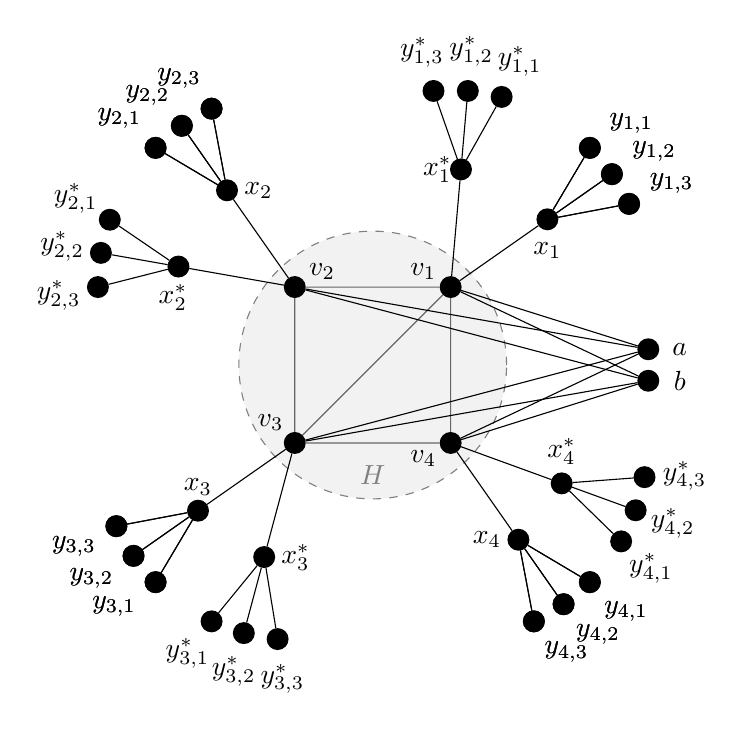
\begin{tikzpicture}					
				%---------- H CORE  --------------- 		
				\node (cent) at (0,0) {};
				\fill[lgray, dashed] (0,0) circle (1.7cm);
				
				
				\foreach \i / \j in {1,2,3,4}
				{
					\path(cent) ++( \i*90-45: 14 mm) node[std]  (v\i) {};
					%					,label={  \i*90-45:$v_{\i}$}
				}	
				
				\draw[mgray](v1)--(v2)--(v3)--(v4)--(v1)--(v3);
				
				\draw[gray, dashed] (0,0) circle (1.7cm);
				\node (H) at (0,-1.4) [color=gray](L){$H$};				
				
				%---------- X Stems  --------------- 
				\foreach \i  in {1,2,3,4}
				{
					\path(v\i) ++( \i*90-55: 15 mm) node[std]  (x\i) {};
					\draw(x\i)--(v\i);
					
					%	\path(v\i) ++( \i*90-55: 25 mm) node[std]  (y\i2) {};
					%	\draw(x\i)--(y\i2);
					%,label={\i*90-45:$x_{\i}$}
					\foreach \j in {1,3}
					{						
						\path(v\i) ++( \i*90-45: 25 mm) node[std,label={ \i*90-65:$y_{\i,1}$}]  (y\i1) {};
						\path(v\i) ++( \i*90-55: 25 mm) node[std,label={ \i*90-75:$y_{\i,2}$}]  (y\i2) {};
						\path(v\i) ++( \i*90-65: 25 mm) node[std,label={ \i*90-85:$y_{\i,3}$}]  (y\i3) {};
						%	\path(x\i) ++( \i*90-105+\j*24: 10 mm) node[std,label={\i*90-105+\j*24:$y_{\i,\j}$}]  (y\i\j) {};
						\draw(x\i)--(y\i1);
						\draw(x\i)--(y\i2);
						\draw(x\i)--(y\i3);
					}					
				}	
				
				
				%---------- X* Stems  --------------- 
				\foreach \i  in {1,2,3,4}
				{
					\path(v\i) ++( \i*85: 15 mm) node[std]  (xs\i) {};
					%	,label={\i*90-45:$x^*_{\i}$}
					\draw(xs\i)--(v\i);
					
					%	\foreach \j in {1,2,3}
					%	{
						%		\path(xs\i) ++( \i*90-85+\j*24: 10 mm) node[std,label={\i*90-85+\j*24:$y^*_{\i,\j}$}]  (ys\i\j) {};
						%		\draw(xs\i)--(ys\i\j);
						%	}					
					
					\path(v\i) ++( \i*85-10: 25 mm) node[std]  (ys\i1) {};
					%				,label={ \i*85-10:$y_{\i,1}^*$}
					\path(v\i) ++( \i*85-12: 30 mm) node   (Lys\i1) {$y_{\i,1}^*$};
					%	\path (v1) ++(150:4mm)  node (Lv1) {$v_{1}$};
					\path(v\i) ++( \i*85: 25 mm) node[std]  (ys\i2) {};
					%				,label={ \i*85:$y_{\i,2}^*$}
					\path(v\i) ++( \i*85: 30 mm) node  (Lys\i2) {$y_{\i,2}^*$};
					\path(v\i) ++( \i*85+10: 25 mm) node[std]  (ys\i3) {};
					%				,label={ \i*85+10:$y_{\i,3}^*$}
					\path(v\i) ++( \i*85+12: 30 mm) node  (Lys\i3) {$y_{\i,3}^*$};
					%	\path(x\i) ++( \i*90-105+\j*24: 10 mm) node[std,label={\i*90-105+\j*24:$y_{\i,\j}$}]  (y\i\j) {};
					\draw(xs\i)--(ys\i1);
					\draw(xs\i)--(ys\i2);
					\draw(xs\i)--(ys\i3);
					
					
				}	
				
				%---------- Z* ------------------		
				\node (z) at (0:35mm) {};		
				
				\foreach \i/\j in {1/90, 2/270}
				{
					\path (z) ++(\j:2mm)  node[std ] (z\i) {};
					
					\foreach \j in {1, 2, 3, 4}
					{
						\draw(z\i)--(v\j);
					}
					
				}	
				
				
				%---------- LABEL FIX------------------
				\path (z1) ++(0:4 mm)  node (La) {$a$};
				\path (z2) ++(0:4 mm)  node (Lb) {$b$};
				
				
				\path (v1) ++(150:4mm)  node (Lv1) {$v_{1}$};
				\path (v2) ++(30:4mm)  node (Lv2) {$v_{2}$};
				\path (v3) ++(140:4mm)  node (Lv3) {$v_{3}$};
				\path (v4) ++(210:4mm)  node (Lxv4) {$v_{4}$};				
				
				\path (x1) ++(270:4mm)  node (Lx1) {$x_{1}$};
				\path (x2) ++(0:4mm)  node (Lx2) {$x_{2}$};
				\path (x3) ++(90:3mm)  node (Lx3) {$x_{3}$};
				\path (x4) ++(180:4mm)  node (Lx4) {$x_{4}$};
				
				\path (xs1) ++(180:3mm)  node (Lxs1) {$x_{1}^*$};
				\path (xs2) ++(260:4mm)  node (Lxs2) {$x_{2}^*$};
				\path (xs3) ++(0:4mm)  node (Lxs3) {$x_{3}^*$};
				\path (xs4) ++(90:4mm)  node (Lxs4) {$x_{4}^*$};
				
				
		\end{tikzpicture}}
		\caption{The graph $G$ constructed from $H$ in Theorem \ref{thm:s:totRom}.}%
		\label{fig:s:trCons}%
	\end{figure}
	%~~~~~~~~~~~~~~~~~~~~~~~~~FIG END~~~~~~~~~~~~~~~~~~~~~~
	
	
	
	%---------------
	We define the family of functions $\mathcal{F}=\{f_1, f_2, \dots, f_n\}$ for $1 \leq k \leq n$ by  
	
	\vspace{-5mm}
	
	\begin{align*}
		f_k(v) = \begin{cases} 2 & \text{ for }v  \in \{x_i, x_i^*\}, i=1,2,\dots,n, \\
			2 	&  \text{ for } v=v_k,\\
			1	& \text{ for } v=v_i, \text{ for } i\neq k,\\
			0&  \text{ for } v\in \{a,b\}.\\
		\end{cases}
	\end{align*}
	
	%$f_k(x_i)=f_k(x_i^*) = 2$ for each $i=1,2, \dots, n$, $f(a)=f(b)=0$, $f_k(v_k)=2$, and $f_k(v_i)=1$ for $i \neq k$.  
	\noindent 
	Then $c(f_k) = 5n+1$, and $f_k$ is  total Roman dominating.  We claim that the family $\mathcal{F}$ are all the least cost total Roman dominating functions of $G$.
	
	Let $g$ be a minimum total Roman dominating function, so that $c(g) \leq c(f_k)$.  To begin, we determine $g(v_i)$.
	Suppose $g(v_i)=0$ for some $i$.   Then, to totally Roman dominate the star $\mathcal{Z}_i$, $\sum_{v\in \mathcal{Z}_i} g(v) \geq 3$, and likewise $\sum_{v\in \mathcal{Z}_i^*} g(v) \geq 3$.  Define a function $g^*$ by
	
	\begin{align*}
		g^*(v) = \begin{cases} f_k(v) & \text{ for } v\in \mathcal{Z}_i \cup \mathcal{Z}_i^*, \\
			1 & \text{ for } v=v_i,\\
			g(v)  & \text{ otherwise.} \\
		\end{cases}
	\end{align*}
	
	
	\noindent Then $g^*$ is a total Roman dominating function of lower cost than $g$, contradicting that $g$ is of minimum cost.  Therefore, $g(v_i) \geq 1$ for each $i$.
	
	Suppose $g(v_i)=1$ for each $v_i$.  Then, to totally Roman dominate $a$ and $b$,  $g(a), g(b) \geq 1$.   Setting $g^*(a)=g^*(b)=0$, and $g^*(v_i)=2$ for any $i$, gives a total Roman dominating function of lower cost.  Therefore, $g(v_i)=2$ for at least one $i\in \{1,2,\dots,n\}$.
	
	
	%yields a total Roman dominating function $g^*$ of lower cost, a contradiction.
	
	
	Next, we determine $g(x_i)$.  Suppose now that	$g(x_i) < 2$.  Then, $\sum_{1\leq j \leq 3} g(y_{i,j}) \geq 3$.    Again, setting $g^*(x_i) = 2$ and $ g^*(y_{i,j}) =0$ for each $1\leq j \leq 3$, gives a total Roman dominating function of lower cost.  Hence $g(x_i)=2$, and similarly, $g(x_i^*)=2$ for each $i$.
	
	
	
	Since  $c(g) \leq c(f_k)$, it now follows easily that $g=f_k$ for some $k \in \{1,2,\dots,n\}$.  
	Thus,  $\gamma_{tR}(G) = 5n+1$, and that	$\mathcal{F}$ consists of all total Roman dominating functions of $G$.  Moreover, the vertex corresponding to $f_i$ in $\gamma_{tR}(G)$ is adjacent to the vertex corresponding to $f_j$ if and only if $v_i$ is adjacent to $v_j$ in $H$.  It follows that $G(\gamma_{tR})\cong H$ as required.	
\end{proof}

	In this chapter, we examined several variations on the $\gamma$-graph.  In each case, with the exception  of the $\gamma_R$-graph, we demonstrated that all graphs are $\pi$-graphs for their respective parameters $\pi$. 
Thus, the natural question to explore is what other parameters $\pi$ are like $\gamma_R$, in that not every graph is a $\pi$-graph?
For example, for the upper irredundance number $IR$, Mynhardt and Roux have shown that not all connected graphs are $IR$-graphs, but that all disconnected graphs are $IR$-graphs \cite{MR22B, MR22A}.	
For remainder of this dissertation we focus on a single such $\gamma$-graph variation, the $i$-graph, which like the $\gamma_R$-graph and the $IR$-graph, is not realizable for all graphs.

